\def\Ponderation{40}
\def\SigleNumero{STT-1000}
\def\NomCours{Probabilités et statstique}
\def\DateEvaluation{26 février 2026}
\def\HeureEvaluation{18 h 30 à 21 h 20}
\def\Session{}
\def\NomEvaluation{Examen 1}

% Ne rien mettre entre les accolades si l'enseignant (ou l'enseignante) est aussi le coordonnateur (ou la coordonnatrice)
\def\Coordonnatrice{}
\def\Coordonnateur{}

% Ne rien mettre entre les accolades s'il y a plus d'une section
\def\Enseignant{}
\def\Enseignante{}

% Ne rien mettre entre les accolades s'il s'agit d'un cours à section unique
% Mettre le nom de chacun des enseignants et enseignantes entre les accolades
% Une case à cocher sera générée pour chacune des sections
\def\SectionA{Anne-Sophie Charest}
\def\SectionB{Julien Miron}
\def\SectionC{}
\def\SectionD{}



\def\Directives{
\begin{enumerate}
\item Matériel autorisé:
\begin{itemize}
\item Calculatrice scientifique {\bf autorisée par la faculté des sciences et de génie};
\item Le feuillet de formules fourni avec l'examen. Celui-ci inclut la table de la loi normale. Veuillez ne rien écrire sur le feuillet de formules.
\end{itemize}
\item Assurez-vous que cette évaluation comporte \numquestions ~exercices répartis sur \numpages{}~pages, pour un total de \numpoints{}~points.\
\item \textbf{Veuillez ne pas dégrafer votre examen.}
\item Vous devez\textbf{ justifier toutes vos réponses} par une démarche claire, sauf pour les questions à choix de réponse.\
\item Pour les questions à choix de réponse et les vrais ou faux, vous pouvez mettre un X, un crochet ($\checkmark$) ou remplir la case.\
\item Vous devez laisser tout ce qui ne servira pas durant l'examen à l'avant de la salle AVANT de rejoindre votre place.\
\item Vous n'avez droit à AUCUN appareil électronique en votre possession durant l'examen.
\item Une fois assis à votre place, vous devez demandez l'autorisation pour vous lever, même si l'examen n'est pas encore commencé, sauf lorsque vous avez terminé l'examen.
\item Dans les 5 dernières minutes de l'examen, il sera interdit de se lever avant que TOUTES les copies n'aient été ramassées.
\end{enumerate}
\begin{itemize}
\item[$\rightarrow$] Le non-respect des consignes 7-8-9 entraînera une pénalité de 10\%.
\end{itemize}
}



\documentclass{Evaluation}
\usepackage{multicol,graphicx}

\printanswers
\begin{document}
\begin{questions}


\pageblanche

%%%%%%%%%%%%%%%% QUESTION MODULE 1 - COMBINATOIRE%%%%%%%%%%%%%%%%


\question[]


On considère l’espace échantillonnal
\[
U = \{a,b,c,d,e,f\}
\]
et les ensembles
\[
A = \{a,b,c\}, \qquad
B = \{b,d,e\}, \qquad
C = \{c,e,f\}.
\]

Calculez les ensembles suivants :\\
\begin{parts}
\part[3]\(A \cup B^c\)
\begin{solution}
On a 
$B^c = \Omega \setminus B = \{a,c,f\}.$
Donc, \[
A \cup B^c = \{a,b,c\} \cup \{a,c,f\} = \{a,b,c,f\}.
\]
\end{solution}

\vspace{6cm}
\part[3] \((A \cup B) \cap C\)   
\begin{solution}
\[
A \cup B = \{a,b,c,d,e\}
\]
\[(A \cup B) \cap C = \{a,b,c,d,e\} \cap \{c,e,f\} = \{c,e\}.
\]
\end{solution}
%\vspace{2cm}
\end{parts}

\vfill

\question[3]
On souhaite modéliser la durée de vie d’une composante informatique par une variable aléatoire continue. On observe que plus la composante est vieille plus le risque de bris à court terme est élevé. Quelle loi est la plus appropriée pour modéliser la durée de vie de cette composante?

\begin{checkboxes}
\choice Une loi exponentielle, car elle modélise bien les pannes aléatoires.
\choice Une loi uniforme, car la durée de vie de la composante est bornée.
\correctchoice Une loi de Weibull, car son taux de panne peut dépendre de l’âge.
\choice Les lois exponentielle et Weibull sont équivalentes dans ce contexte.
\end{checkboxes}
\vspace{3cm}

\pageblanche
\question[10]


Une station de radio possède une banque de \(14\) chansons.
\begin{itemize}
\item \(4\) chansons sont du même artiste (artiste A);
\item les \(10\) autres chansons sont toutes d’artistes différents, et différents de A.
\end{itemize}

On choisit au hasard \(5\) chansons distinctes pour une liste de lecture. Quelle est la probabilité que la liste contienne \emph{exactement deux} chansons de l’artiste A?

\begin{solution}
Le nombre total de choix possibles de \(5\) chansons parmi \(14\) est
\[
\binom{14}{5}.
\]

Pour avoir exactement deux chansons de l’artiste A :
\begin{itemize}
\item on choisit \(2\) chansons parmi les \(4\) de l’artiste A : \(\binom{4}{2}\);
\item on choisit \(3\) chansons parmi les \(10\) autres : \(\binom{10}{3}\).
\end{itemize}

Le nombre de choix favorables est donc
\[
\binom{4}{2}\binom{10}{3}.
\]

La probabilité demandée vaut
\[
\mathbb{P}(\text{exactement 2 de A})
=
\frac{\binom{4}{2}\binom{10}{3}}{\binom{14}{5}}.
\]

On peut simplifier numériquement :
\[
\binom{4}{2}=6,\qquad \binom{10}{3}=120,\qquad \binom{14}{5}=2002,
\]
donc
\[
\mathbb{P}=\frac{6\cdot 120}{2002}=\frac{720}{2002}=\frac{360}{1001}.
\]

\[
\boxed{\mathbb{P}=\frac{360}{1001}.}
\]
\end{solution}


 \pageblanche



 \pageblanche
%%%%%%%%%%%%%%%% QUESTION MODULE 1 - PROBABILITÉS%%%%%%%%%%%%%%%%

\pageblanche
\question[]

Un sac contient 40 billes rouges, 40 billes vertes et 20 billes bleues.
Sur certaines de ces billes, une étoile a été dessinée.
Nous savons que la probabilité de choisir une bille sans étoile parmi les billes rouges est de $0,875$, la probabilité de choisir une bille qui est verte et qui a une étoile est de $0,1$ et la probabilité de choisir une bille qui a une étoile parmi les billes bleues est de $0,5$.

En utilisant les événements suivants:

\begin{itemize}
    \item R: la bille est rouge
    \item V: la bille est verte
    \item B: la bille est bleue
    \item E: une étoile est dessinée sur la bille
\end{itemize}

\begin{parts}
    \part[3] Tracez le diagramme de Venn qui représente cette situation. \textit{Vous n'avez qu'à identifier les événements et \textbf{l'espace échantillonnal}. Il n'est pas nécessaire d'inscrire les probabilités.}
\begin{solution}

    \begin{tikzpicture}[scale=1, font=\small]

% --- Paramètres (faciles à ajuster) ---
\def\W{9}   % largeur de Omega
\def\H{5}   % hauteur de Omega
\def\xA{3}  % séparation 1 (entre R et V)
\def\xB{6}  % séparation 2 (entre V et B)

% --- Dessin (on "clip" pour que tout reste dans Omega) ---
\begin{scope}
  \clip (0,0) rectangle (\W,\H);

  % Partition R, V, B : 3 bandes disjointes qui couvrent Omega
  \fill[red!18]   (0,0) rectangle (\xA,\H);
  \fill[green!18] (\xA,0) rectangle (\xB,\H);
  \fill[blue!18]  (\xB,0) rectangle (\W,\H);

  % Evénement E par-dessus (semi-transparent) qui intersecte R, V, B
  \fill[gray!40, opacity=0.35] (\W*0.52,\H*0.55) ellipse [x radius=\W*0.43, y radius=\H*0.28];
  \draw[thick, gray!70!black]  (\W*0.52,\H*0.55) ellipse [x radius=\W*0.43, y radius=\H*0.28];

  % Lignes de séparation de la partition
  \draw[thick] (\xA,0) -- (\xA,\H);
  \draw[thick] (\xB,0) -- (\xB,\H);

  % (Optionnel) petites étiquettes dans les intersections
  \node at (\W*0.17,\H*0.60) {\scriptsize $E\cap R$};
  \node at (\W*0.50,\H*0.35) {\scriptsize $E\cap V$};
  \node at (\W*0.83,\H*0.60) {\scriptsize $E\cap B$};
\end{scope}

% Contour de Omega (par-dessus tout)
\draw[very thick, rounded corners=6pt] (0,0) rectangle (\W,\H);
\node[anchor=south west] at (0,0) {$\Omega$};

% Étiquettes des événements de la partition
\node at (\xA/2, \H*0.15) {$R$};
\node at ((\xA+\xB)/2, \H*0.15) {$V$};
\node at ((\xB+\W)/2, \H*0.15) {$B$};

% Étiquette de E
\node[gray!70!black] at (\W*0.82,\H*0.87) {$E$};

\end{tikzpicture}
\end{solution}
    \vspace{3.5cm}

    \part[8] Si vous avez pigé une bille avec une étoile, quelle est la probabilité que celle-ci soit bleue?

    \begin{solution}
        On cherche $P(B|E)$

        \begin{align*}
            P(B|E)&=\frac{P(B\cap E)}{P(E)}\\
            &=\frac{P(E|B)P(B)}{P(E\cap R)+P(E\cap V)+P(E\cap B)}\\
            &=\frac{P(E|B)P(B)}{P(E|R)P(R)+P(E|V)P(V)+P(E|B)P(B)}\\
            &=\frac{0,5\times 0,2}{(1-0,875)\times 0,4+0,1+0,5\times 0,2}\\
            &=\frac{2}{5}
        \end{align*}
    \end{solution}
\vfill
\part  \begin{subparts}
        \subpart[1] Les événements R et V sont indépendants.
        
        \begin{oneparcheckboxes}
            \choice Vrai
            \correctchoice Faux
        \end{oneparcheckboxes}

        \subpart[1] Les événements R et E sont indépendants.
        
        \begin{oneparcheckboxes}
            \choice Vrai
            \correctchoice Faux
        \end{oneparcheckboxes}


        \subpart[1] Les événements R, V et B forment une partition de l'espace échantillonnal.
        
        \begin{oneparcheckboxes}
            \correctchoice Vrai
            \choice Faux
        \end{oneparcheckboxes}
    \end{subparts}
    \vspace{0.5cm}
\end{parts}

\pageblanche
%%%%%%%%%%%%%%%% QUESTION MODULE 2 - VA %%%%%%%%%%%%%%%%
\question\label{densite} Soit $X$ une variable aléatoire continue de densité $f_X$ définie ci-dessous.

\begin{minipage}[]{7cm}{
\vspace{0cm}
\[ f_X(x) = \begin{cases}
\vspace{0.2cm}
\displaystyle \frac{1}{18} & \mbox{si } 0\leq x < \displaystyle \frac{a}{5}, \\
\vspace{0.2cm}
\displaystyle \frac{1}{9} & \mbox{si } \displaystyle\frac{a}{5}\leq x \leq \displaystyle a, \\
\displaystyle 0 & \mbox{sinon.}
\end{cases} \]
    }
\end{minipage}
 \hspace{10mm}
\begin{minipage}[]{7cm}{
\vspace{0cm}
\begin{tikzpicture}[xscale=0.45, yscale=15]

% Axes
\draw[->, thick] (-1,0) -- (11.8,0) node[right] {$x$};
\draw[->, thick] (0,-0.002) -- (0,0.14) node[above] {$f(x)$};

% Graduations x
  \draw (2,0) -- (2,-0.002) node[below] {\small $\displaystyle 
  \sfrac{a}{5}$};
    \draw (10,0) -- (10,-0.002) node[below] {\small $\displaystyle 
  a$};

% Niveaux y
\draw (-0.15,1/18) -- (0,1/18) node[left] {\small $\frac{1}{18}$};
\draw (-0.15,1/9)  -- (0,1/9)  node[left] {\small $\frac{1}{9}$};

% Segments de la densité
\draw[very thick] (-1,0) -- (0,0);
\draw[very thick] (10,0) -- (11.8,0);
\draw[very thick] (0,1/18) -- (2,1/18);
\draw[very thick] (2,1/9) -- (10,1/9);

% Points (NODES -> pas déformés par xscale/yscale)
\node[circle, draw=black, inner sep=0pt, minimum size=4pt] at (0,0) {};
\node[circle, fill=black, inner sep=0pt, minimum size=4pt] at (0,1/18) {};
\node[circle, draw=black,  inner sep=0pt, minimum size=4pt] at (2,1/18) {}; % ouvert
\node[circle, fill=black, inner sep=0pt, minimum size=4pt] at (2,1/9) {};
\node[circle, fill=black, inner sep=0pt, minimum size=4pt] at (10,1/9) {};
\node[circle, draw=black, inner sep=0pt, minimum size=4pt] at (10,0) {};

\end{tikzpicture}
    }
\end{minipage}

\textit{Utilisez cette densité pour répondre aux parties (a) et (b).}

\vspace{0.5cm}
\begin{parts}
    \part[4] Que vaut $a$?

    \begin{solution}
        On veut que l'aire totale sous la courbe donne 1. On peut faire l'intégrale ou la somme des deux rectangles. 

        \begin{align*}
            1&=\sfrac{a}{5}\times \sfrac{1}{18}+(a-\sfrac{a}{5}\times \sfrac{1}{9}\\
            1&=\sfrac{a}{90}+\sfrac{4a}{45}\\
            1&=\frac{9a}{90}\\
            10&=a
        \end{align*}
    \end{solution}
\vspace{5cm}
    \part[5] Quelle est la probabilité que $X$ prenne une valeur entre $\displaystyle \frac{a}{10}$ et $\displaystyle \frac{a}{2}$? \textit{Si vous n'avez pas trouvé la valeur de $a$, vous pouvez donner votre réponse en fonction de $a$.}

    \begin{solution}
        On peut encore faire l'intégrale entre les deux points ou calculer l'aire des deux rectangles formés. 

        \begin{align*}
            P(\sfrac{a}{10}<X<\sfrac{a}{2})&=P(1<X<5)\\
            &=(2-1)\times \sfrac{1}{18}+(5-2)\times \sfrac{1}{9}\\
            &=\sfrac{1}{18}+\sfrac{1}{3}\\
            &= \frac{7}{18}
        \end{align*}
    \end{solution}

\vfill
\pagesuivante{\ref{densite}}
\pageblanche
\suite{\ref{densite}}

Voici une autre densité. Utilisez-la pour répondre à la partie (c).

\begin{minipage}[]{7cm}{
\vspace{0cm}
\[ f_Y(y) = \begin{cases}
\vspace{0.2cm}
\displaystyle \frac{1}{180} & \mbox{si } 0\leq y < \displaystyle 20, \\
\vspace{0.2cm}
\displaystyle \frac{1}{90} & \mbox{si } 20\leq y \leq \displaystyle 100, \\
\displaystyle 0 & \mbox{sinon.}
\end{cases} \]
    }
\end{minipage}
 \hspace{10mm}
\begin{minipage}[]{7cm}{
\vspace{0cm}
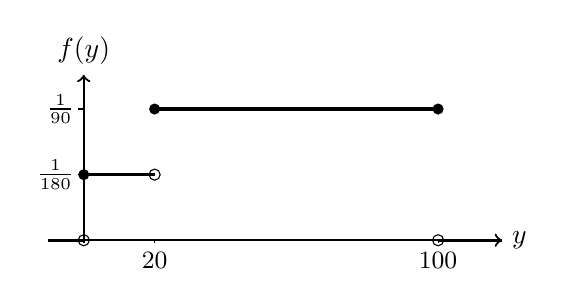
\begin{tikzpicture}[xscale=0.45, yscale=15]

% Axes
\draw[->, thick] (-1,0) -- (11.8,0) node[right] {$y$};
\draw[->, thick] (0,-0.002) -- (0,0.14) node[above] {$f(y)$};

% Graduations x
  \draw (2,0) -- (2,-0.002) node[below] {\small $20$};
    \draw (10,0) -- (10,-0.002) node[below] {\small $100$};

% Niveaux y
\draw (-0.15,1/18) -- (0,1/18) node[left] {\small $\frac{1}{180}$};
\draw (-0.15,1/9)  -- (0,1/9)  node[left] {\small $\frac{1}{90}$};

% Segments de la densité
\draw[very thick] (-1,0) -- (0,0);
\draw[very thick] (10,0) -- (11.8,0);
\draw[very thick] (0,1/18) -- (2,1/18);
\draw[very thick] (2,1/9) -- (10,1/9);

% Points (NODES -> pas déformés par xscale/yscale)
\node[circle, draw=black, inner sep=0pt, minimum size=4pt] at (0,0) {};
\node[circle, fill=black, inner sep=0pt, minimum size=4pt] at (0,1/18) {};
\node[circle, draw=black,  inner sep=0pt, minimum size=4pt] at (2,1/18) {}; % ouvert
\node[circle, fill=black, inner sep=0pt, minimum size=4pt] at (2,1/9) {};
\node[circle, fill=black, inner sep=0pt, minimum size=4pt] at (10,1/9) {};
\node[circle, draw=black, inner sep=0pt, minimum size=4pt] at (10,0) {};

\end{tikzpicture}
    }
\end{minipage}


\part[5] Quelle est l'espérance de $Y$?

\begin{solution}
\begin{align*}
    E(Y)&=\int_{-\infty}^{\infty}yf_Y(y)dy\\
    &= \int_0^{20}\frac{x}{180}dx+\int_{20}^{100}\frac{x}{90}dx\\
    &=\frac{1}{360}[x^2]_{0}^{20}+ \frac{1}{180}[x^2]_{20}^{100}\\
    &= \frac{10}{9}+\frac{160}{3}\\
    &=\frac{490}{9}
\end{align*}    
\end{solution}
\end{parts}



%%%%%%%%%%%%%%%% QUESTION MODULE 3 -  %%%%%%%%%%%%%%%%
 \pageblanche 

\question[]

Une voiture est stationnée sans avoir payé. Chaque jour, indépendamment des autres jours, il y a une probabilité \(p=0{,}15\) qu’elle reçoive une contravention.
On suppose qu’au plus une contravention peut être donnée par jour.
Le coût d’une contravention est de \(65\$\). Le coût d’un permis de stationnement mensuel est de \(180\$\).


\begin{parts}
\part[4] Quelle est la probabilité que la voiture ne reçoive \emph{aucune} contravention au cours des \(7\) premiers jours?
\begin{solution}
Sur \(7\) jours, le nombre de contraventions $X$ suit une loi binomiale :
\[
X \sim \text{Bin}(7,0{,}15).
\]
Donc
\[
\mathbb{P}(X=0)=\binom{7}{0}(0{,}15)^0(0{,}85)^7=(0{,}85)^7.
\]   
\end{solution}

\vspace{6cm}
\part[4] Après combien de jours s’attend-on, en moyenne, à recevoir la première contravention?
\begin{solution}
 Le nombre de jours avant la première contravention suit une loi géométrique de paramètre \(p=0{,}15\).
Ainsi, le nombre moyen de jours avant la première contravention est
\[
\frac{1}{p}=\frac{1}{0{,}15}=\frac{20}{3}\approx 6{,}67\ \text{jours}.
\]   
\end{solution}

\vspace{6cm}
\part[4] En moyenne, après combien de jours s’attend-on à ce que le total des contraventions atteigne ou dépasse \(180\$\)?
\begin{solution}
    Atteindre ou dépasser \(180\$\) nécessite au moins \(3\) contraventions, car
\[
2\times 65=130<180
\qquad \text{et} \qquad
3\times 65=195\ge 180.
\]

On cherche donc le nombre moyen de jours pour recevoir \(3\) contraventions.

Le nombre de jours nécessaires pour obtenir \(r=3\) succès, lorsque chaque jour est un essai indépendant de probabilité \(p=0{,}15\), suit une loi de Pascal (binomiale négative).
Pour cette loi, l’espérance du nombre d’essais nécessaires pour obtenir \(r\) succès est
\[
\mathbb{E}(\text{jours})=\frac{r}{p}.
\]

Ainsi,
\[
\mathbb{E}(\text{jours})=\frac{3}{0{,}15}=20.
\]

\[
\boxed{\text{En moyenne, cela devrait prendre } 20 \text{ jours.}}
\]
\end{solution}
\end{parts}

\vspace{1cm}




 \pageblanche

%%%%%%%%%%%%%%%% QUESTION MODULE 4 - PAS LOI NORMALE %%%%%%%%%%%%%%%%


\question[]

Dans un projet de cartographie, un drone envoie automatiquement des relevés de position vers un serveur. Les relevés sont reçus indépendamment les uns des autres, à un taux constant au cours du temps. On suppose que le nombre de relevés reçus suit un processus de Poisson de taux \(\lambda = 1{,}5\) relevé par heure. Charles surveille la réception des relevés.

\begin{parts}
\part[4]  Charles souhaite aller dîner pendant \(40\) minutes.
Quelle est la probabilité qu’il ne manque \emph{aucun} relevé pendant son absence? 
\begin{solution}
Sur \(40\) minutes, soit \(t=\frac{40}{60}=\frac{2}{3}\) heure, le nombre de relevés reçus suit une loi de Poisson
de paramètre
\[
\lambda t = 1{,}5 \times \frac{2}{3} = 1.
\]
Ainsi,
\[
\mathbb{P}(\text{aucun relevé}) = \mathbb{P}(N=0) = e^{-1}.
\]
\end{solution}

\vspace{6cm}
\part[4] S’il vient de recevoir un relevé, en moyenne combien de temps a-t-il
avant de recevoir le \emph{prochain} relevé?
\begin{solution}
Le temps d’attente avant la réception du prochain relevé suit une loi exponentielle
de paramètre \(\lambda = 1{,}5\).
L’espérance vaut
\[
\frac{1}{\lambda} = \frac{1}{1{,}5} = \frac{2}{3}\ \text{heure},
\]
soit environ \(40\) minutes.

\end{solution}

\vspace{6cm}
\part[4] Pour rédiger son article, Charles a besoin de  \(100\) relevés. En moyenne, combien de temps faudra-t-il pour obtenir ces \(100\) relevés?
\begin{solution}
Le temps nécessaire pour recevoir \(100\) relevés suit une loi gamma
de paramètre de forme \(k=100\) et de taux \(\lambda = 1{,}5\).
L’espérance vaut
\[
\frac{k}{\lambda} = \frac{100}{1{,}5} \approx 66{,}7\ \text{heures}.
\]
\end{solution}
\end{parts}

 \pageblanche

%%%%%%%%%%%%%%%% QUESTION MODULE 4 - LOI NORMALE %%%%%%%%%%%%%%%%
\question[]\label{gruyere} Un producteur de Gruyère sait que le poids d'une de ses meules de fromage, $X$, est une variable aléatoire qui suit une loi normale d'espérance $\mu=30$ kg et de variance $\sigma^2 = 9$ kg$^2$. 
Il doit envoyer 144 meules à un festival. 
Le transporteur lui chargera 1500\$, à condition que le poids moyen des 144 meules soit inférieur ou égal à $30,295$ kg. 
Dans le cas contraire, il lui chargera 2000\$.

\begin{parts}
    \part[6] Quelle est la probabilité que le transporteur lui charge 1500\$?
    \begin{solution}
        $X\sim \mathcal{N}(30; 9)$. Donc $\overline{X}\sim \mathcal{N}(30;\sfrac{9}{144})$

        \begin{align*}
            P(\overline{X}<30,295)&=P\left(\frac{\overline{X}-30}{3/12}<\frac{30,295-30}{3/12}\right)\\
            &=P\left(Z<1,18 \right)\\
            &=0,881
        \end{align*}
    \end{solution}
    \vspace{15cm}
    \part[3] Quelle est l'espérance du prix qu'il en coûtera au producteur pour envoyer ses meules?
\begin{solution}
    Soit $W$ la variable aléatoire qui prend 1 si le poids moyen est plus petit que 30,295 et 0 sinon. $W\sim Bernoulli(0,881)$ et $E(W)=0,881$. La variable aléatoire du prix est $U=W\times 1500 + (1-W) \times 2000$. $E(U)=1559,5$
     
\end{solution}
\vfill
\pagesuivante{\ref{gruyere}}
\pageblanche
\suite{\ref{gruyere}}
\part[6] Le producteur sait que la quantité de lait nécessaire pour produire 0,5 kilogramme de Gruyère est d'espérance $6$ litres et de variance $4$ litres$^2$. Quelle est la probabilité qu'il lui faille moins de 415,36 litres pour produire une meule de 32 kilogrammes?
\begin{solution}
    Il faut 64 fois 0,5 kg pour produire 32 kg. Ici $X_1,\hdots,X_{64}$ représentent la quantité de lait pour 500 grammes et $E(X_i)=6$, $V(X_i)=9$, pour $i=1,\hdots,64$. Comme la loi des $X_i$ n'est pas spécifiée, on utilise le TCL, avec $T=X_1+\hdots+X_{64}\approx \mathcal{N}(64\times 6; 64 \times 4)$.

    \begin{align*}
        P(T<415,36)&=P\left(\frac{T-384}{16}<\frac{415,36-384}{16}\right)\\
        &\approx P(Z<1,96)\\
        &=0,975
    \end{align*}
\end{solution}
\end{parts}


\pageblanche
%%%%%%%%%%%%%%%% QUESTION MODULE 5 - LOI CONJOINTE %%%%%%%%%%%%%%%%

\question Soit l'expérience aléatoire qui consiste à lancer deux dés réguliers à 6 faces. 
On définit les variables aléatoires $X$ et $Y$ qui sont respectivement la somme et la différence absolue des deux dés.

Voici les probabilités conjointes de $X$ et $Y$.

% (optionnel) \usepackage{graphicx}  % pour \resizebox
% (optionnel) \usepackage{xfrac}     % pour \sfrac si tu en utilises ailleurs

\begin{center}
%\resizebox{\textwidth}{!}{%

\begin{tabular}{cc|*{11}{c}|}
$p(x,y)$ & & \multicolumn{11}{c|}{$x$}  \\
 & & $2$ & $3$ & $4$ & $5$ & $6$ & $7$ & $8$ & $9$ & $10$ & $11$ & $12$ \\
\hline
 & $0$ & $\sfrac{1}{36}$ & 0 & $\sfrac{1}{36}$ & 0  & $\sfrac{1}{36}$ &  0 & $\sfrac{1}{36}$ & 0  & $\sfrac{1}{36}$ & 0  & $\sfrac{1}{36}$ \\
$y$ & $1$ & 0  & $\sfrac{1}{18}$ &  0 & $\sfrac{1}{18}$ &   0& $\sfrac{1}{18}$ & 0  & $\sfrac{1}{18}$ &   0& $\sfrac{1}{18}$ & 0 \\
 & $2$ &  0 &  0 & $\sfrac{1}{18}$ &  0 & $\sfrac{1}{18}$ & 0  & $\sfrac{1}{18}$ & 0  & $\sfrac{1}{18}$ &0   & 0  \\
 & $3$ &  0 &  0 & 0  & $\sfrac{1}{18}$ & 0  & $\sfrac{1}{18}$ & 0  & $\sfrac{1}{18}$ & 0  &  0 & 0  \\
 & $4$ &  0 &  0 &  0 &0   & $\sfrac{1}{18}$ &  0 & $\sfrac{1}{18}$ &  0 & 0  &  0 & 0  \\
 & $5$ &  0 &  0 &   0& 0  &0   & $\sfrac{1}{18}$ & 0  & 0  &  0 & 0  &  0 \\
\hline

\end{tabular}

%}
\end{center}

\begin{parts}
\part[4] Quelle est la probabilité que la somme des dés soit inférieure à 5 et que leur différence soit inférieure à 3?
\begin{solution}
    On peut simplement faire la somme des $p(x,y)$ où $x<5$ et $y<3$. $P(X<5\cap Y<3)=\sfrac{1}{36}+\sfrac{1}{36}+\sfrac{1}{18}+\sfrac{1}{18}=\sfrac{1}{6}$
\end{solution}
\vspace{4cm}

\part[6] Quelle est l'espérance de $Y$, sachant que $X=6$?
\begin{solution}
\begin{align*}
    E(Y|X=6)&=0\times \frac{\sfrac{1}{36}}{\sfrac{1}{36}+\sfrac{1}{18}+\sfrac{1}{18}}+ 2 \times \frac{\sfrac{1}{18}}{\sfrac{1}{36}+\sfrac{1}{18}+\sfrac{1}{18}}+ 4\times \frac{\sfrac{1}{18}}{\sfrac{1}{36}+\sfrac{1}{18}+\sfrac{1}{18}}\\
    &=0\times \sfrac{1}{5} + 2 \times \sfrac{2}{5}+4\times \sfrac{2}{5}\\
    &= 2,4
\end{align*}

\end{solution}
\vfill

\part[4] Les variables aléatoire $X$ et $Y$ sont indépendantes. \textit{Une réponse sans bonne justification n'aura aucun point, même si elle est bonne.}

\begin{oneparcheckboxes}
    \choice Vrai
    \correctchoice Faux
\end{oneparcheckboxes}

\textbf{Justification:}
\begin{solution}
    N'importe quelle combinaison $p(x,y)\neq p(x)p(y)$
\end{solution}
\vspace{4cm}
\end{parts}



\pageblanche
\end{questions}
\end{document} 
